%!TEX root=Principal.tex
\chapter{\emph{FRAMEWORK} PARA AUTOAVALIAÇÃO DO COMPORTAMENTO SOCIAL DO ROBÔ}
\label{cap:proposta}

Os capítulos anteriores apresentam uma revisão da literatura apontando que a existência de robôs em ambientes sociais torna-se cada vez mais comum no dia-a-dia das pessoas. Como qualquer produto existente no mercado, é necessário que esses robôs tragam uma boa experiência aos usuários que convivem com ele. Entretanto, as técnicas difundidas em interação humano computador, que tem o objetivo de aumentar a experiência boa do usuário em produtos tecnológicos, não têm sido aplicadas de maneira adequada por pesquisadores na área de robótica social, de serviço e assistiva~\cite{alenljung:2017}.

Com esse cenário em mente, essa tese apresenta um \emph{framework} baseado em teoria de experiência do usuário focado na usabilidade para aumentar o conforto da presença do robô. No processo apresentado como guia para a construção e evolução do \emph{framework}, assim como a criação de novos projetos em robótica, algumas técnicas serão utilizadas, como: (I) Personas que serão para o robô a base de classificação do perfil do usuário; (II) Heurísticas de Nielsen adaptadas para a interação humano robô, que servem como guia para o robô avaliar seu desempenho; e (III) \emph{Proxemics}, a teoria de proximidade (vide seção~\ref{cap:proxemics}), que estuda o comportamento de agentes sociais de acordo com a distância entre si.

De acordo com a literatura apresentada, a cultura da pessoa influência diretamente o comportamento de uma pessoa em ambientes sociais. Isso significa que algumas reações apresentadas por pessoas no ambiente social são influenciadas pelo seu local de nascimento, pelos locais onde viveu e, consequentemente, pela sua experiência de vida. Contudo, fatores como a experiência de vida e cultura são difíceis de avaliar apenas através da observação. Conseguir fazer com que uma pessoa tenha liberdade para contar esse tipo de informação necessita de interações de longo prazo, podendo levar meses até compreender toda história dessa pessoa.

Contudo, o robô sendo um produto tecnológico pode utilizar técnicas que são capazes de aumentar a efetividade da interação. Não havendo assim, a necessidade de conhecer por completo a história de vida do indivíduo em questão. Técnicas oriundas da área de interação humano computador, tem o objetivo de deixar o sistema mais fácil de usar e acima de tudo aumentar a experiência, a satisfação do usuário ao utilizá-lo. Para que o robô possa realizar essa classificação e raciocínio sobre as informações que existem no ambiente alguns passos são apresentados ao longo deste capítulo.

A seção~\ref{sec:robo} apresenta em detalhes o robô utilizado para essa pesquisa. Com base no robô disponível, estabelece as ações que são possíveis para ele executar. Na sequência dois questionários foram preparados, o primeiro aplicado anteriormente ao teste e o segundo após. O intuito do primeiro questionário é estabelecer o perfil do usuário referente a questões de aderência a tecnologia, contato prévio com robôs e sobre a cultura que ele se identifica. O questionário pós-teste possui informações declaradas sobre o conforto e avaliação do comportamento do robô durante a interação.

Com os questionários definidos, foram selecionados 39 pessoas para participar do teste de interação com o robô, de acordo com o cenário descrito na seção~\ref{sec:cenario}. Os testes foram executados com o comportamento do robô de maneira aleatória, ou seja, sem nenhuma preocupação com a experiência do usuário neste momento. Coletados os perfis e informações dos usuários, é realizado uma preparação e normalização dos dados para que o algoritmo QG-SIM possa realizar o agrupamento dos perfis similares, conforme o processo apresentado por \citeonline{masiero:2013b}. A partir dos grupos gerados pelo algoritmo QG-SIM, é realizado o processo de criação de Personas~\cite{masiero:2013, masiero:2013b}.

Personas criadas, o próximo passo é estabelecer a criação de uma estrutura de nós no formato de rede bayesiana causa-efeito com camadas referentes as Personas, heurísticas de Nielsen adaptadas, comportamento do robô e efeitos sobre conforto e desconforto do usuário. Essa rede bayesiana é responsavél pelo mecanismo de auto-avaliação do robô. O mecanismo proposto possui uma estrutura mínima de nós, que refere-se ao ponto de partida do \emph{framework}. Essa estrutura pode evoluir para quantos nós forem necessários em uma avaliação mais precisa para a tomada de decisão e adaptação do comportamento do robô para mitigar o desconforto do usuário na presença do robô. Ao final, um conjunto de variáveis são propostos como ponto para futuras investigações e aprimoramento do \emph{framework} entregue por essa tese.

O restante deste capítulo apresenta em detalhes os passos da proposta acima descrita. Ao final do capítulo é apresentado a visão completa da metodologia onde é realizado uma síntese do processo como um todo e das técnicas aplicadas nele.

\section{Comportamentos do Robô}
\label{sec:comportamento-robo}
O robô escolhido para os experimentos possui uma série de características que auxiliam a interação social e serviço domésticos, uma vez que ele foi construído para atender a competição de robótica RoboCup@Home~\cite{robocup:2015}. Com base nos atuadores de interação existentes (vide seção~\ref{sec:sensores}), foram mapeados as variáveis de comportamento do robô. A tabela~\ref{tab:variaveisvalores} apresenta as variáveis, compostas por seus respectivos valores.

\begin{table}[!ht]
	\caption{Variáveis de Comportamento do Robô}
	\label{tab:variaveisvalores}
	\centering
	\begin{tabular}{c | c}
		\hline
		Variável & Valor \\
		\hline
		& Olá Curto \\
		Gestos & Olá Longo \\
		& Apontar \\
		\hline
		Estilo de Fala & Educada \\
		& Autoritaria \\
		\hline
		& Nervosa com Cor Vermelha \\
		& Nervosa com Cor Azul \\
		Estilo de Face & Neutra \\
		& Feliz \\
		& Triste \\
		& Surpresa e Corada \\
		\hline
		Proximidade & Entre Pública e Social \\
		& Entre Pessoal e Íntima \\
		\hline
		Velocidade & Rápida \\
		& Devagar \\
		\hline
		Rotação no próprio eixo & Rápida \\
		& Devagar \\
		\hline
	\end{tabular}
	\smallcaption{Fonte: O autor.}
\end{table}

Além das variáveis direcionadas aos atuadores do robô, a tabela~\ref{tab:variaveisvalores} apresenta a variável de proximidade entre o robô e o ser humano. Essa variável é importante, pois auxilia a determinar o comportamento de reação da pessoa para um mesmo gesto do robô. Por exemplo, se o robô encontra-se próximo da pessoa, entre as zonas Pessoal e Íntima, um gesto amplo pode gerar um desconforto maior do que o mesmo gesto ocorrendo entre as zonas Pública e Social. Com as variáveis definidas e comportamentos implementados no robô é importante agora trabalhar com os questionários pré e pós testes.

\section{Questionários para o Teste}
\label{sec:questionarios}

\section{Rede Bayesiana para Auxiliar na Aproximação do Robô}
\label{sec:rede-bayesiana}

Analisando os sensores disponíveis no robô utilizado para implementação e execução dos testes dessa tese (vide seção~\ref{sec:robo}) e as variáveis apresentadas nas seções~\ref{sec:variaveiscomportamentais} e \ref{sec:variaveisrobo}, optou-se por utilizar variáveis mínimas e com o menor número de sensores, para auxiliar no diagnóstico e tomada de decisão do robô. A quantidade de menor número de sensores é justificada devido a facilidade de implementar em qualquer tipo de robô com o menor custo. As variáveis foram segmentadas para que tomada de decisão feita pelo robô fosse automática, sem necessidade de controla-lo de qualquer maneira. Apesar dessa segmentação das variáveis na implementação da rede bayesiana, as mapeadas na seção~\ref{sec:extracaocaracteristicas} estão documentadas para que sejam incluídas em trabalhos futuros, melhorando assim o processo de análise comportamental do indíviduo, assim como outras aqui não contempladas. As variáveis que serão utilizadas são:

\begin{itemize}
	\item POS: posicionamento do robô dentro da zona de proximidade social da pessoa, apresentada no capítulo~\ref{cap:proxemics} através da figura~\ref{fig:proximityzones};
	\item VEL: velocidade de aproximação do robô em relação a pessoa;
	\item VOL: volume de emissão de som, realizado pelo robô;
	\item GES: amplitude do gesto do robô em relação a pessoa;
	\item FACE: expressão facial apresentada pelo robô durante a aproximação;
	\item AFASTOU: se a pessoa se afastou do robô após sua tentativa de aproximação;
	\item NEG\_FACE: se a pessoa apresentou uma expressão facial negativa durante a tentativa de aproximação do robô;
	\item NEG\_CORP: se a pessoa apresentou uma expressão corporal negativa durante a tentativa de aproximação do robô;
\end{itemize}

Para cada uma das variáveis aleatórias é necessário o mapeamento dos domínios. Os domínios são importantes para definir quais os possíveis valores que cada variável pode assumir, além de limitar o escopo do trabalho de maneira a atingir o seu objetivo. O domínio de cada variável aleatória apresentada é:

\begin{itemize}
	\item POS = \{publica, social, pessoal, íntima\}
	\item VEL = \{rápido, devagar\}
	\item VOL = \{alto, baixo, mudo\}
	\item GES = \{longo, curto, ausente\}
	\item FACE = \{feliz, neutra, nervoso\}
	\item AFASTOU = \{verdadeiro, falso\}
	\item NEG\_FACE = \{verdadeiro, falso\}
	\item NEG\_CORP = \{verdadeiro, falso\}
\end{itemize}

As variavéis que representam a reação do usuário (\{AFASTOU, NEG\_FACE, NEG\_CORP\}) possuem o domínio binário, pois o intuito é apenas saber se algum fator gerou uma reação negativa do ser humano durante a interação. As demais várias necessitam de um domínio maior, pois a intenção é investigar quais os fatores que levaram a reação negativa do ser humano.

Com a definição das variáveis aleatórias e seus respectivos domínios, foi possível estabelecer um grafo acíclico orientado, uma rede bayesiana, partindo do princípio de que POS é o nó pai que tem influência sobre todos os outros. Ele foi escolhido como nó pai, pois é a causa principal dos demais efeitos da rede, que possui mais dois níveis. Em um nível intemediário de nós temos as variávies \{VEL, VOL, GES, FACE\}, que são variáveis dependentes exclusivamente das ações do robô e possuem uma independência condicional dado o pai POS. Por fim, as três variáveis que representam as reações do ser humano, que são independentes condicionais dado os pais \{POS, VEL, VOL, GES, FACE\}. As variáveis \{AFASTOU, NEG\_FACE, NEG\_CORP\} também são chamadas de nós de efeito, que querem ser observados durante o processo de interação humano robô. A figura~\ref{fig:rb} apresenta a rede bayesiana formada com base na hierarquia definida.

\begin{figure}[ht!]
	\centering
	\begin{minipage}{0.8\textwidth}
		\caption{Rede bayesiana construída para auxiliar no diagnóstico e tomada de decisão da aproximação ao indivíduo.}
		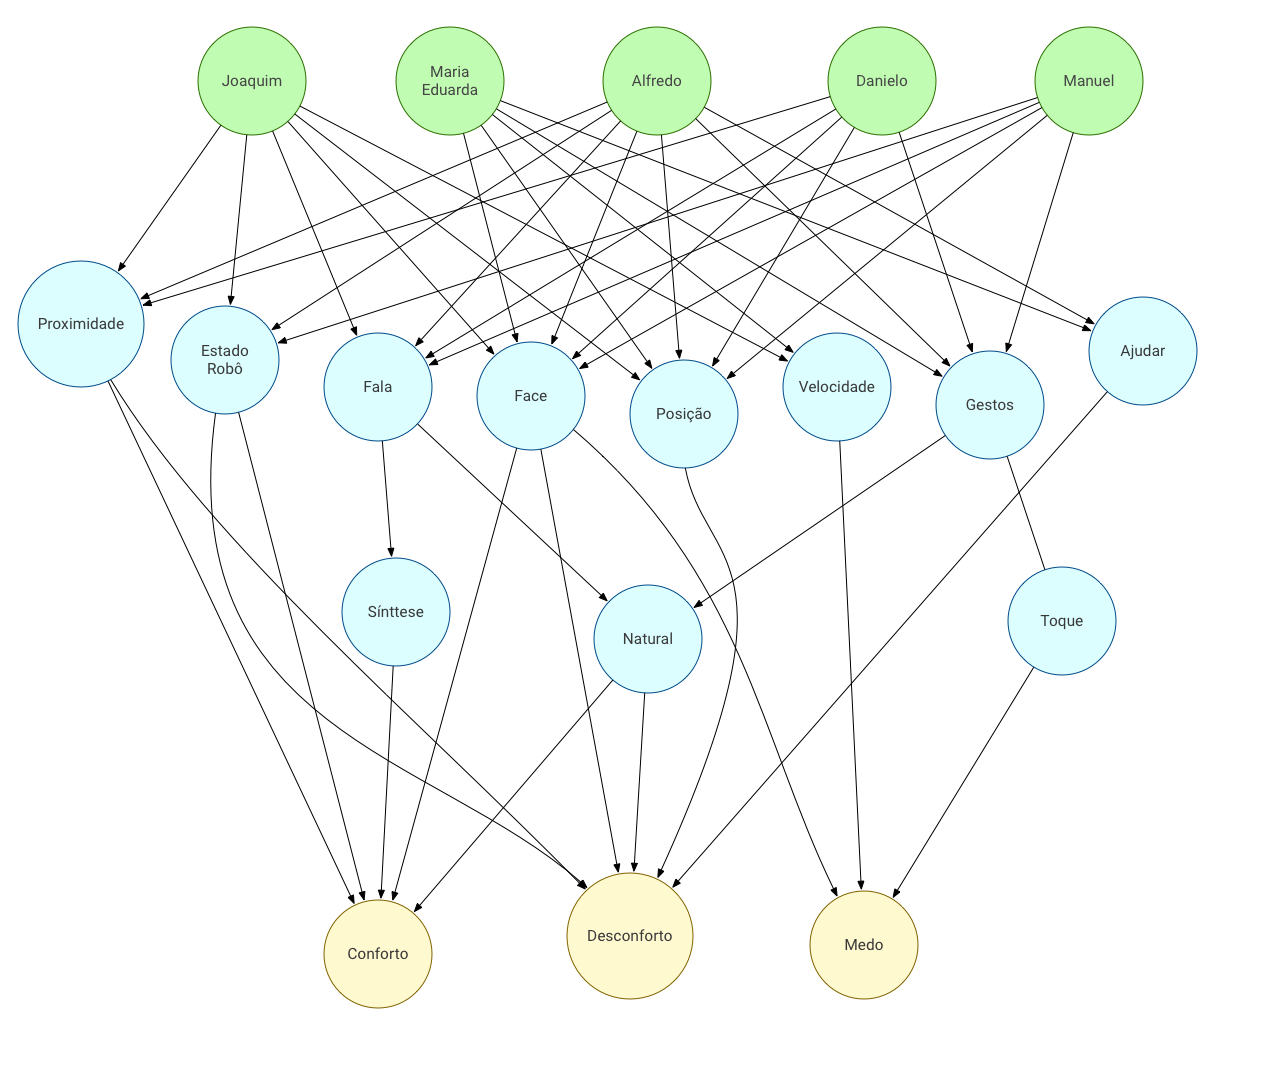
\includegraphics[width=\textwidth]{rb-thesis.png}
		\smallcaption{Fonte: Autor.}
		\label{fig:rb}
	\end{minipage}
\end{figure}

A partir de agora é preciso formalizar a rede bayesiana em formato de probabilidades, para que seja possível compreender cada um dos cálculos de inferência e diagnóstico realizados pelo mecanismo de tomada de decisão do robô durante a tarefa de aproximação do indivíduo. As equações~\ref{eq:1}, \ref{eq:2}, \ref{eq:3}, \ref{eq:4}, \ref{eq:5}, \ref{eq:6}, \ref{eq:7} e \ref{eq:8} representam as probabilidades da rede bayesiana para cada uma das variáveis aleatórias mapeadas.

\begin{equation}
	\label{eq:1}
	P(POS)
\end{equation}

\begin{equation}
	\label{eq:2}
	P(VEL|POS)
\end{equation}

\begin{equation}
	\label{eq:3}
	P(VOL|POS)
\end{equation}

\begin{equation}
	\label{eq:4}
	P(GES|POS)
\end{equation}

\begin{equation}
	\label{eq:5}
	P(FACE|POS)
\end{equation}

\begin{equation}
	\label{eq:6}
	P(AFASTOU|POS, VEL, VOL, GES, FACE)
\end{equation}

\begin{equation}
	\label{eq:7}
	P(NEG\_FACE|POS, VEL, VOL, GES, FACE)
\end{equation}

\begin{equation}
	\label{eq:8}
	P(NEG\_CORP|POS, VEL, VOL, GES, FACE)
\end{equation}

É importante ressaltar que o efeito a ser medido é a reação do ser humano, pois é o principal interessado em toda interação com o robô, já que é um robô com tarefas em ambientes sociais, domésticos e assistivos. A grande preocupação em manter o foco no ser humano é por que os trabalhos apresentados no capítulo~\ref{cap:proxemics} tem o foco apenas na execução da tarefa pelo robô e em seu comportamento. As reações dos seres humanos são colocadas em segundo plano, nesses trabalhos.

\section{Extração das Características}
\label{sec:extracaocaracteristicas}

Como apresentado no capítulo \ref{cap:proxemics}, existem diversas variáveis que podem auxiliar na extração de um perfil comportamental do indivíduo. \emph{Proxemics} tornam possível a extração de fatores sobre a distância social entre o indivíduo e o robô. Esses fatores podem variar não só entre a posição física dos dois agentes, mas também na posição do corpo dos indivíduos, como por exemplo, a orientação dos ombros e troco em relação a posição do robô. Outro fator significante é a fixação entre olhares, este pode auxiliar o processo que determina o início e o fim de uma interação. O olhar também auxilia na determinação de quem são os principais indivíduos na interação. Além disso, pode-se empregar o reconhecimento de expressões faciais para auxílio na análise do quanto a situação é confortável para o indivíduo, ou o quanto ele aprecia a interação. Pode existir uma avaliação em tempo real das reações deste indivíduo durante todo o processo de interação. Outra técnica que pode ser utilizada na análise de conforto na interação é a avaliação da emoção através da voz da pessoa, ou através do uso de equipamento de eletroencefalografia~(EEG), porém este último é um método mais invasivo já que exige a adição de um equipamento na pessoa que interage com o robô.

É possível empregar diversos sensores que auxiliam a leitura e quantificação dessas variáveis. Sensores de captura de marcações de movimento, como Microsoft\textregistered\ Kinect\textregistered\ ou o ASUS\textregistered\ Xtion\textregistered, são utilizados para quantificar os valores comportamentais obtidos através das variáveis, que envolvem distância entre agentes e orientação de membros do indivíduo. Para realizar o reconhecimento de expressões faciais utiliza-se uma câmera de video, podendo assim executar uma leitura da face da pessoa em tempo de execução. As variáveis referentes a questão da fixação dos olhares dos agentes para identificar o início e o fim da interação, podem ser obtidas através de ambos sensores, sendo possível determinar a orientação da cabeça e torso do indivíduo, além de também a direção do olhar da pessoa para o robô. A voz do indivíduo para análise da emoção na interação é obtida através de um microfone direcional ou um arranjo de microfones, que amplifica a capacidade de percepção do robô em relação ao ambiente e a pessoa que interage com ele. A figura~\ref{fig:capturacaracteristicas} apresenta a ilustração do processo de extração das características do indivíduo.

\begin{figure}[ht!]
	\centering
	\begin{minipage}{0.8\textwidth}
		\caption{Processo para a extração das características do indivíduo.}
		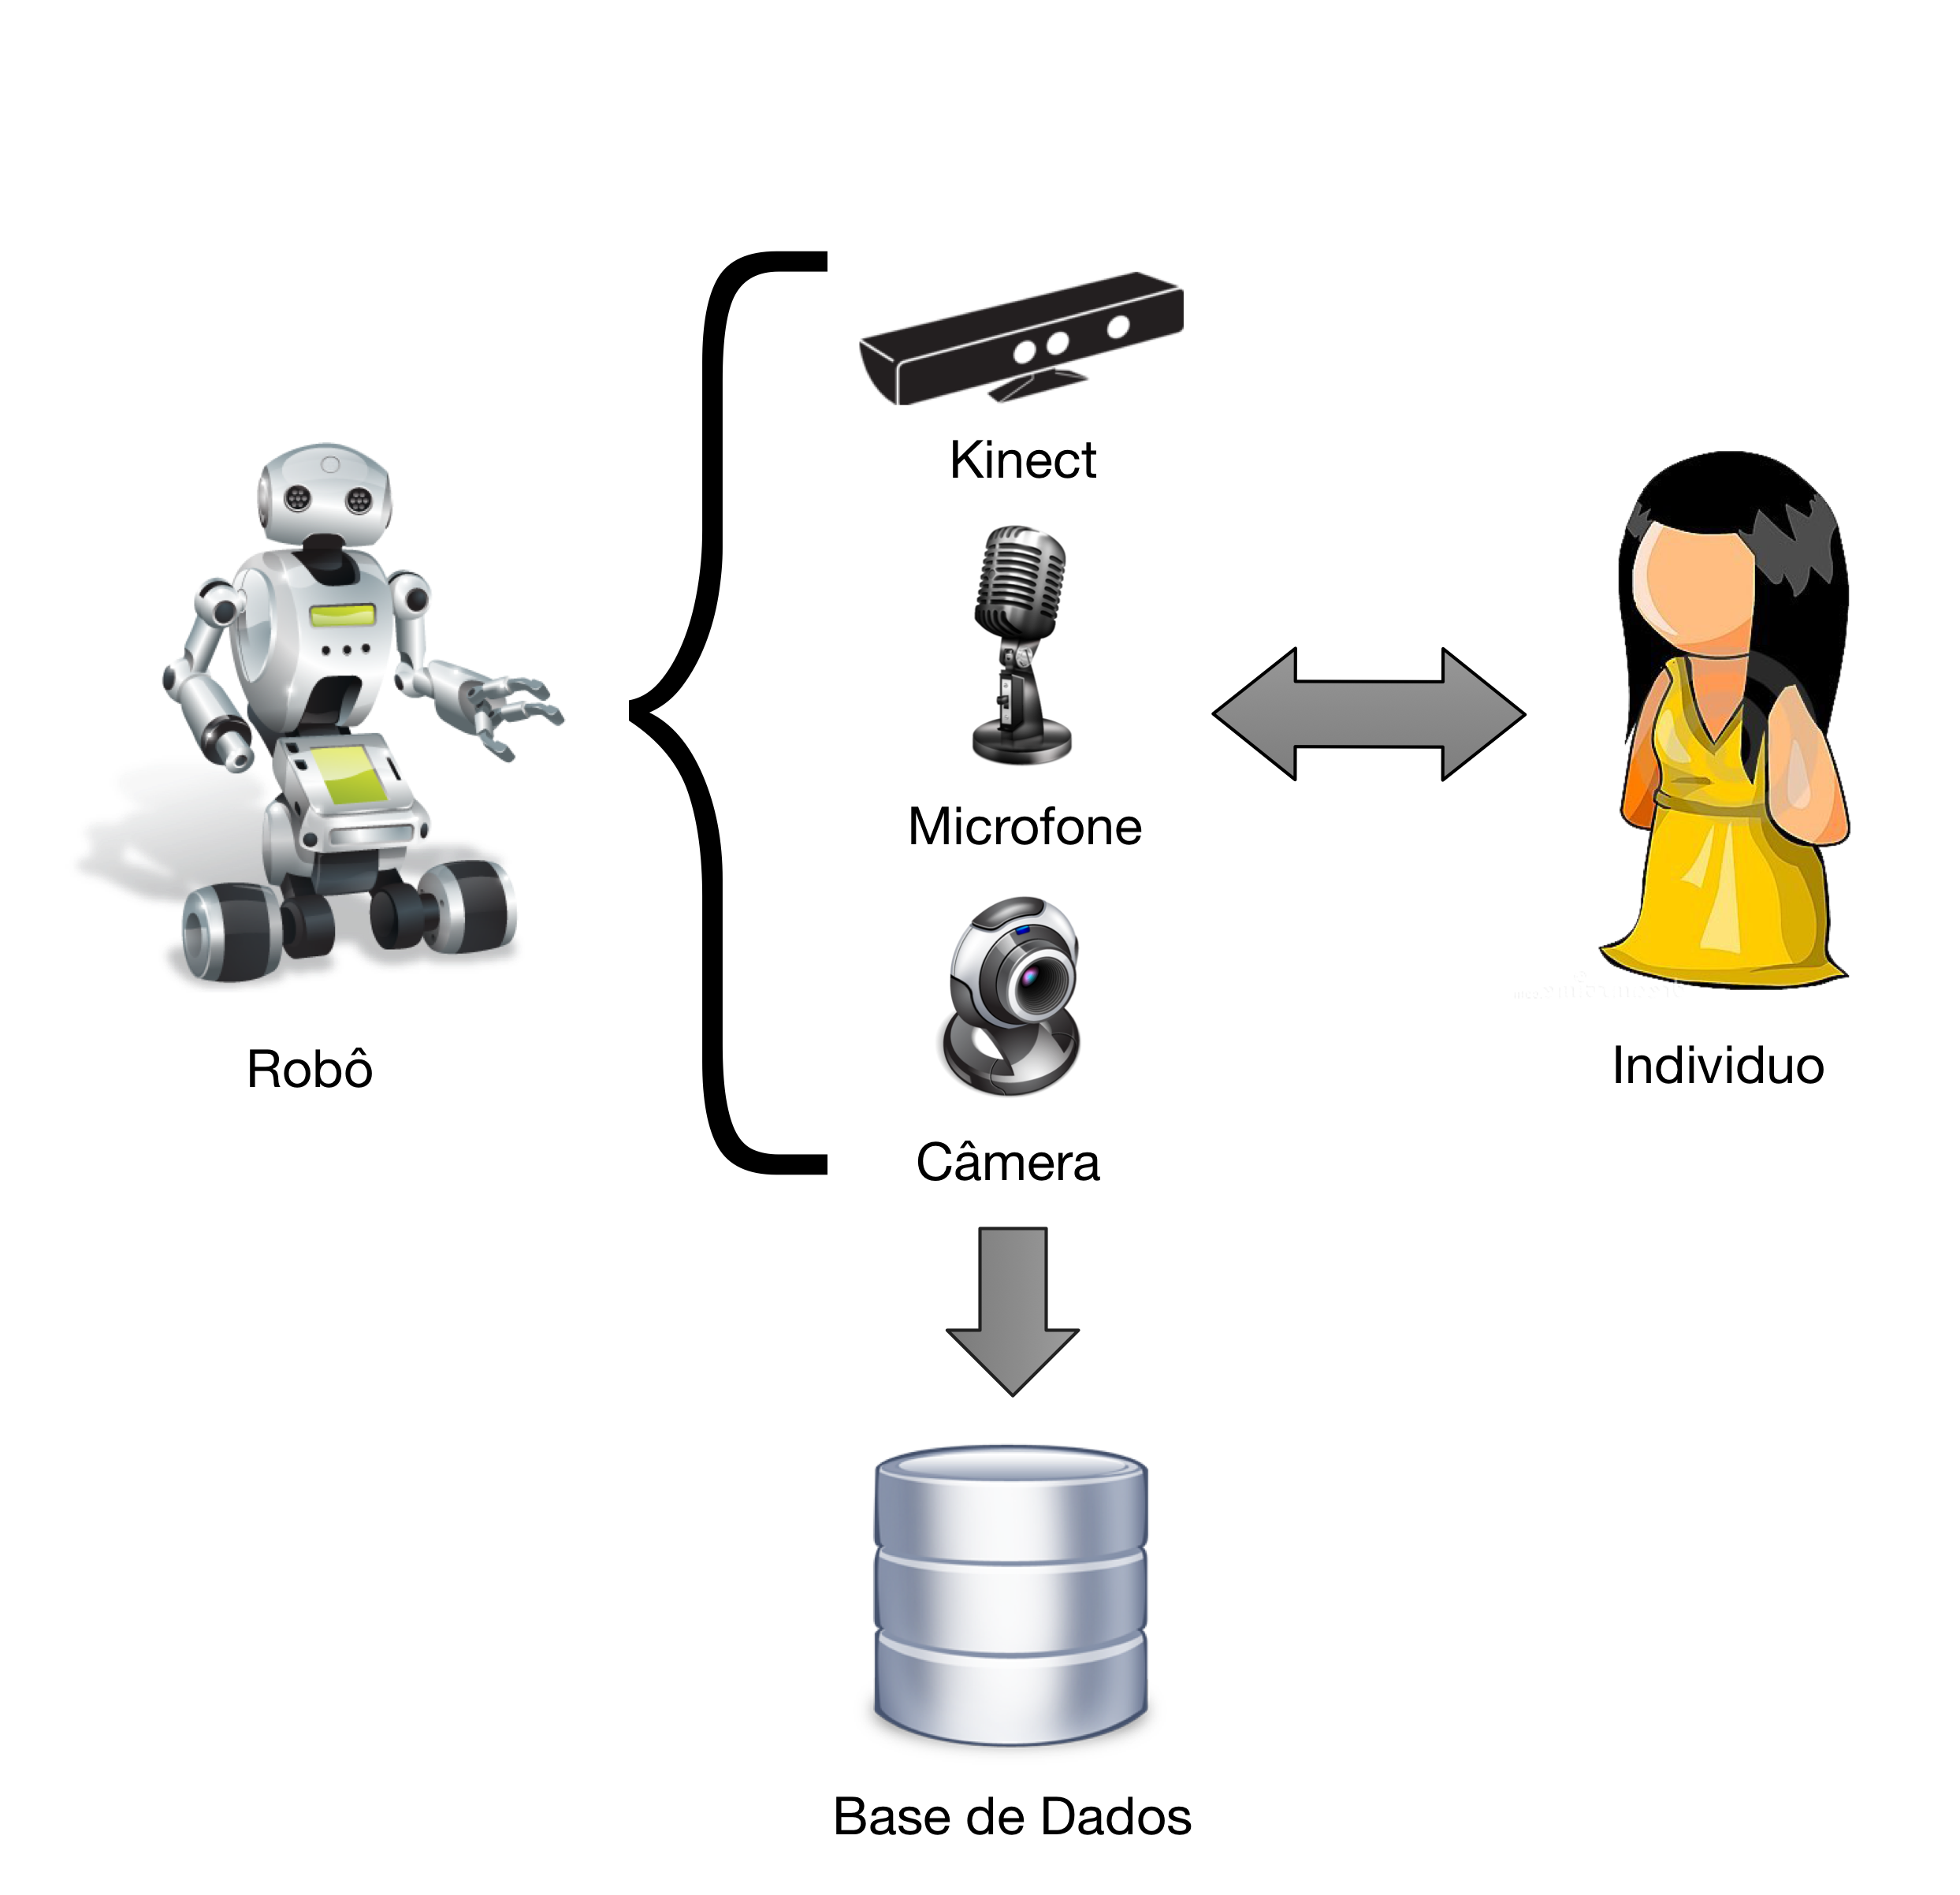
\includegraphics[width=\textwidth]{captura_carac_individuo.png}
		\smallcaption{Fonte: Autor.}
		\label{fig:capturacaracteristicas}
	\end{minipage}
\end{figure}

No processo apresentado pela figura \ref{fig:capturacaracteristicas}, o robô utiliza os sensores para identificar o indivíduo e analizar a reação dele durante a aproximação física. Durante a aproximação, o robô utiliza um componente de \emph{log} que armazena todos os valores das variáveis que são utilizadas para analisar, posteriormente, o comportamento do robô (ação) e do indivíduo (reação) em um banco de dados. As variáveis são apresentadas em detalhes nas seções \ref{sec:variaveisindivíduo} e \ref{sec:variaveisrobo}.

Com as informações armazenadas inicia-se o processo de análise através de métodos estátisticos, que auxiliam a determinar as variáveis que mais apresentam correlação dentro do problema estudado. A extração de perfis comportamentais das pessoas é realizado e possibilita identificar os grupos de perfis comportamentais obtidos na interação. Os perfis podem ser utilizados em projetos futuros de robótica social, de serviço e assistiva, porém nessa tese eles irão compor o nó principal da rede bayesiana desenvolvida. Esse tipo de informação também é útil para identificar a relação de comportamento entre robôs e humanos. Deve-se lembrar que as informações sobre o comportamento são direcionadas por um cenário de interação~\cite{jung:1991}, então um mesmo indivíduo pode apresentar comportamento diferente em cenários de atuação diferentes.

Dessa forma, as variáveis aplicadas ao comportamento tem dependência do cenário de interação, porém as informações das variáveis etnográficas como idade, experiência computacional, sexo, local de origem, etnia, entre outras, são independentes do cenário. Existem alguns algoritmos na área de visão computacional que são capazes de identificar algumas variáveis etnográficas de maneira automática \cite{yang:2007, shan:2012, ylioinas:2012, samadi:2013, amaral:2014}, porém para o trabalho desta tese, a coleta dessas informações será realizada através de um questionário pré e pós interação já que esses algoritmos não fazem parte do objetivo principal do trabalho. As informações obtidas através do questionário serão inseridas no banco de dados complementando as informações de comportamento, que são obtidas, de forma separada, através da interação entre o ser humano e o robô através dos cenários de interação.

Na seção~\ref{sec:variaveisindivíduo} são detalhados os conjuntos de variáveis etnográficas e comportamentais com uma breve explicação dos objetivos esperados de cada uma das variáveis coletadas. A seção~\ref{sec:variaveisrobo} detalha as variáveis que serão consideradas para o perfil do robô, apresentando também uma explicação sobre os objetivos de cada uma das variáveis. Essas seções são consideradas como um mapa de variáveis importante para estudos comportamentais em interação humano-robô social. Pode-se inserir mais ou remover algumas variáveis durante a aplicação na construção de robôs autônomos sociais. A seção~\ref{sec:rede-bayesiana} apresentará melhor a seleção realizada por esta tese e como é aplicado no mecanismo de inferência comportamental.

\subsection{Selecionando Variáveis do indivíduo}
\label{sec:variaveisindivíduo}

Essa seção apresenta os conjuntos de variáveis que são consideradas como a base de informações para desenvolvimento de estudos em interação humano-robô social. Dois conjuntos são apresentados, o conjunto de variáveis etnográficas, seguido pelo conjunto de variáveis comportamentais que é o principal foco deste trabalho.

\subsubsection{Conjunto de Variáveis Etnográficas}
\label{sec:variaveisetnograficas}

O objetivo das variáveis etnográficas é identificar qual a experiência social e computacional de cada indivíduo. Além da experiência, também pode-se obter informações sobre a idade, gênero, local de nascimento ou origem do indivíduo. Todas essas informações são relevantes para verificar a existência de uma possível relação entre as variáveis etnográficas e comportamentais, além da relevância cultural para estabalecer uma aproximação e posteriormente uma interação social. A lista apresentada a seguir define as variáveis etnográficas e uma breve explicação sobre o significado de cada uma das variáveis.

\begin{enumerate}
	\item \textbf{Idade}: informa a idade do indivíduo.
	\item \textbf{Gênero}: informa o sexo biológico do indivíduo.
	\item \textbf{Local de Nascimento}: informa qual o local de nascimento do indivíduo. Essa variável auxiliará a determinar a base cultural do indivíduo.
	\item \textbf{Etnia}: informa a origem da família do indivíduo. Outra variável que auxilia na determinação da base cultural do indivíduo.
	\item \textbf{Quantidade de \emph{Gadgets}}: informa a quantidade de \emph{gadgets} que o indivíduo possui, ajudando a identificar qual a experiência e o contato dele com a tecnologia.
	\item \textbf{Contato prévio com Robôs}: informa apenas se o indivíduo já possuiu algum contato com robôs. Auxiliará a determinar o contato com a tecnologia, principalmente com robôs que poderá influenciar no seu comportamento durante a interação.
	\item \textbf{Tipos de Robôs}: informa quais são os tipos de robôs que o indivíduo teve contato. Os tipos poderão ser robôs \emph{Pet}, Humanoides, Androides, Móveis, entre outros. Essa variável é um complemento da variável ``Contato prévio com Robôs''.
	\item \textbf{Quantidade de cidades visitadas}: informa a quantidade de cidades que o indivíduo já visitou além da sua cidade natal. É importante para identificar o contato com outros tipos de cultura. Isso poderá influenciar no comportamento definido por sua cultura.
	\item \textbf{Quantidade de cidades que morou}: informa a quantidade de cidades que o indivíduo já morou além da sua cidade natal. É importante para identificar a vivência com outros tipos de cultura. Isso poderá influenciar no comportamento definido por sua cultura.
	\item \textbf{Quantidade de países visitadas}: informa a quantidade de países que o indivíduo já visitou além da sua cidade natal. É importante para identificar o contato com outros tipos de cultura. Isso poderá influenciar no comportamento definido por sua cultura.
	\item \textbf{Quantidade de países que morou}: informa a quantidade de países que o indivíduo já morou além da sua cidade natal. É importante para identificar a vivência com outros tipos de cultura. Isso poderá influenciar no comportamento definido por sua cultura.
\end{enumerate}

Em diversos trabalhos da seção \ref{sec:proxemicsihr}, onde a questão cultural do indivíduo é abordada, são discutidos que influência a cultura provê sobre o comportamenteo do o indivíduo. Contudo, a cultura é tratada como a origem do indivíduo, por exemplo, no trabalho de \citeonline{eresha:2013}. Entretanto, esta tese acredita que a questão cultural na vida de uma pessoa é mais abrangente. Ela está relacionada a experiência adquirida ao longo de sua vivência social, como por exemplo, países e cidades que o indivíduo visitou e viveu, o meio ao qual ele está inserido, sua profissão, entre outras informações. Dessa forma, o conjunto de variáveis apresentado na lista acima tem como objetivo mapear de forma abstrata a experiência social do indivíduo, com o intuito de verificar se o comportamento é menos dependente da origem do indivíduo e mais dependente de sua experiência prévia de vida.

As informações apresentadas nessa seção serão adquiridas através de questionários pré interação. Em trabalhos futuros poderão ser aplicados estudos para identificar essas informações de maneira interativa através do próprio robô.

\subsubsection{Conjunto de Variáveis Comportamentais}
\label{sec:variaveiscomportamentais}

Variáveis comportamentais tem como principal objetivo identificar o comportamento do indivíduo dentro do cenário exigido por uma determinada tarefa. Nessa tese o comportamento está diretamente relacionado com cenários de interação social. As variáveis comportamentais são coletadas a partir de informações sobre as posições corporais e expressões faciais do indivíduo, tornando possível uma análise com base em teorias de linguagem corporal e de microexpressões. As análises realizadas a partir da linguagem corporal, tem por base o trabalho apresentado por \citeonline{lambert:2008}. O conjunto de variáveis comportamentais apresentados nessa seção não são utilizadas apenas para extrair o perfil do indivíduo, mas também para avaliar se a ação realizada pelo robô gerou uma reação positiva ou negativa no indivíduo. A lista apresentada a seguir define as variáveis comportamentais obtidas através da literatura e uma breve explicação sobre o objetivo de cada uma das variáveis.

\begin{enumerate}
	\item \textbf{Expressões Faciais}: é possível identificar se a reação do indivíduo foi positiva ou negativa, a partir de uma ação do robô. Existem seis expressões bases que combinadas formam diversas outras~\cite{bihan:2014}. Contudo, nesse trabalho será considerado apenas as seis expressões bases classificadas em dois grupos: expressões faciais positivas e expressões faciais negativas. O intuito dessa variável é realizar a avaliação da ação do robô com base nas expressões faciais do indivíduo.
	\item \textbf{Tempo de Transição entre as Zonas Sociais}: identificar o tempo que o indivíduo ficou confortável com a presença do robô a medida que esse diminuiu a distância entre eles.
	\item \textbf{Frequência do Olhar em direção ao Robô}: identificar se o indivíduo mantém o olhar ao robô, sendo possível saber se a interação está continua ou não. Isso pode influenciar se o robô está interagindo de maneira confortável ao indivíduo ou se esse está incomodado com a presença do robô.
	\item \textbf{Tempo do Olhar}: é possível mensurar o interesse do indivíduo durante a interação através do tempo que ele permanece com o olhar fixo no robô. Quanto maior o tempo do olhar, maior o interesse na interação do indivíduo.
	\item \textbf{Orientação dos ombros}: Auxilia a mensurar o interesse do indivíduo durante a interação, analisando se os ombros possuem a mesma orientação que a cabeça e também uma orientação em direção ao indivíduo que interage com o robô. Além disso, é possível determinar através do alinhamento do quadril com o ombro do indivíduo o ângulo de inclinação de seu torso. A inclinação do torso auxilia a identificar o interesse do indivíduo na interação, para isso basta verificar se ele está inclinado em direção ao robô para determinar um interesse positivo.
	\item \textbf{Orientação do quadril}: Auxilia a mensurar o interesse do indivíduo durante a interação. A orientação do quadril em direção ao robô ou na direção oposta auxilia a determinar o grau de interesse do indivíduo na interação. Quando mais alinhado à direção do robô, maior o interesse do indivíduo na interação.
	\item \textbf{Estilo da Voz}: é importante, pois pode determinar a reação que o indivíduo terá após a interação via áudio com o robô. Além disso, é possível determinar se o indivíduo está confortável ou não durante a interação, analisando o tom de sua voz ao responder o robô. Nesse trabalho, será considerado somente o canal de resposta ao indivíduo. A análise do tom da voz do indivíduo não será considerado nesta tese e ficará para trabalhos futuros de aprimoramento do componente de análise comportamental em IHR.
\end{enumerate}

As variáveis apresentadas acima podem auxiliar na descoberta do interesse em relação a interação. Algumas delas, como as que envolve o olhar, podem necessitar de equipamentos mais específicos para obter uma melhor acurácia na captura. Outras variáveis necessitam de muitas técnicas e estudos direcionados para trazer a interação à um nível mais natural, como o caso da voz. Dessa forma, escolher quais variáveis trabalhar tem influência não só sobre o estudo realizado, como também nos equipamentos embarcados no robô. Tais equipamentos, podem influenciar em sua aparência e consequentemente na interação. Essas variáveis que influenciam sobre o robôs são apresentadas na seção~\ref{sec:variaveisrobo} a seguir.

\subsection{Selecionando as Variáveis para o Robô}
\label{sec:variaveisrobo}
Além das variáveis referentes ao perfil do indivíduo, deve-se considerar também as informações sobre o robô uma vez que sua aparência pode influenciar na reação das pessoas durante a interação~\cite{hegel:2009}. Coletar as variáveis do robô pode auxiliar a identificar quais são os principais fatores que tornam a interação humano-robô desconfortável ou menos natural ao ser humano. Dessa forma, definiu-se um conjunto de variáveis que pudessem caracterizar da melhor maneira fatores do robô, referente a sua aparência, que influenciam na interação social. Esse conjunto de variáveis é apresentado a seguir:

\begin{enumerate}
	\item \textbf{Altura}: A altura do robô para identificar a influência da diferença entre alturas de robôs e humanos.
	\item \textbf{Volume}: O volume ocupado pelo robô pode influenciar no conforto da interação, uma vez que quando o robô atingir uma zona social mais próxima do indivíduo pode causar uma sensação claustrofóbica a ele.
	\item \textbf{Tipo do Robô}: Segundo \citeonline{choi:2014}, robôs possuem dois tipos: Autônomos e Tele-operados. Essa variável define o quanto de intervenção humana é necessário para que o robô possa executar a tarefa objetivo.
	\item \textbf{Classificação do Robô}: Segundo \citeonline{dobra:2014} classificar um robô é uma tarefa muito complexa e pode envolver diversas variáveis. Dessa forma, para essa tese será considerado uma classificação mais simples. O robô deve ser classificado como: fixo, móvel com rodas, móvel bípede, móvel quadrupede, móvel com manipuladores. Outras classificações podem ser inseridas conforme a necessidade e inclusão de novos robôs.
	\item \textbf{Aparência Física}: Essa variável descreve se o robô possui uma aparência amigável ou agressiva.
	\item \textbf{Nível de Ruído}: Determina qual o nível de ruído que os atuadores do robô podem gerar de tal forma, que possa influenciar na interação humano-robô. Como exemplo, pode-se citar o Big Dog~\footnote{http://www.bostondynamics.com/robot\_bigdog.html}, da Darpa Robotics, que é movido através de um motor diesel e seus atuadores pneumáticos e hidráulicos apresentam um alto grau de ruído.
\end{enumerate}

Além das variáveis que definem as características, é necessário também o mapeamento das ações que o robô irá executar para que exista uma análise das informações após a reação do indivíduo. As variáveis que compõem as informações do perfil comportamental do robô são:

\begin{enumerate}
	\item \textbf{Aproximação}: Forma de aproximação do robô ao indivíduo. Pode ser classificada entre rápida, devagar, brusca ou suave.
	\item \textbf{Movimentação do Manipulador}: Caso exista um manipulador deve descrever como é feita a movimentação do manipulador em direção ao usuário. A classificação pode ser feita entre brusca e suave; ou em relação a sua amplitude, como longo e curto.
	\item \textbf{Estilo de Voz}: Ao emitir algum tipo de som o robô deverá manter um estilo de voz para que seja possível simbolizar qual o tipo de mensagem ele deseja falar. A classificação será feita de maneira simplificada, considerando apenas se é um estilo educado ou agressivo.
	\item \textbf{Volume de Voz}: Ao emitir um som, o robô deve saber qual o volume adequada considerando a interação, ambiente e distância do segundo agente. Uma classificação simples pode ser utilizada, como por exemplo, alto e baixo.
	\item \textbf{Expressão Facial}: Ao iniciar o contato visual com o indivíduo, pode ocorrer diversas expressões do robô na tentativa de manter o conforto do indivíduo durante o processo de interação. Simplificando as expressões, de maneira similar ao apresentado na seção~\ref{sec:variaveiscomportamentais}, são consideradas apenas dois tipos de expressões realizadas pelo robô: amistoso e não-amistoso. As expressões faciais do robô serão executadas através do \emph{tablet} acoplado nele, conforme descrito na seção~\ref{sec:robo}.
\end{enumerate}

As variáveis comportamentais do robô são definidas com o objetivo de executar uma tarefa de abordagem para estabelecer uma interação, ou seja, uma aproximação inicial do ser humano. Caso seja necessário deve-se adicionar novas variáveis a esse conjunto e essa adição não afetará ao método apresentado como uma solução para este problema. O conhecimento prévio da pessoa, um reencontro, não será considerado nessa tese, deixando assim como trabalhos futuros.
